\noindent Thus far, we have diagonalized the Klein-Gordon Hamiltonian
\begin{equation}
\hat{H}_{KG} = \frac{1}{2} \int d^3 x \left( \hat{\pi}^2 (x) + (\nabla \hat{\phi}(x))^2 + m^2 \hat{\phi}^2(x) \right) = \int \frac{d^3 p}{(2\pi)^3} \hat{a}_p^\dagger \hat{a}_p
\end{equation}

\noindent And used this to construct the unitary operator that allows us to study the dynamics of Klein-Gordon's solution to Schr\"odinger's equation in the Heisenberg picture
\begin{equation}
\hat{U} = e^{-i\hat{H}_{KG} t}.
\end{equation}

\noindent We found the spatial solutions $\hat{\phi}(x)$, in the Schr\"odinger picture, for the Klein-Gordon equation, to be the position field operators
\begin{equation}
\hat{\phi} (x) = \int \frac{d^3 p}{(2\pi)^3} \frac{1}{\sqrt{2 \omega_p}} \left( \hat{a}_p e^{i p \cdot x} + \hat{a}_p^\dagger e^{-i p \cdot x} \right)
\end{equation}

\noindent \textbf{Notation:} The spatial 3-vectors of position $x$ and momentum $p$ are no longer bold-faced, and the spacetime 4-vectors will be bold-faced, such that 
\begin{align}
\textbf{x} &= (x^0, x) &= (t,x) &= (x^0, x^1, x^2, x^3) \\
\textbf{p} &= (p_0, p) &= (\omega_p, p) &= (x^0, x^1, x^2, x^3) .
\end{align}

\noindent These solutions are represented in the Heisenberg picture via
\begin{equation}
\hat{\phi}(t, x) = \hat{U}^\dagger \hat{\phi}(x) \hat{U} = e^{i \hat{H}_{KG} t} \hat{\phi}(x) e^{-i \hat{H}_{KG} t}.
\end{equation}

\noindent We still need to complete the (projective) unitary representation of the Poincar\'e group, including translations, boosts, and rotations, since we are doing \textit{relativistic} quantum field theory.  \\

\noindent The next step here is to check that $\hat{\phi}(t,x)$ respects causality, such that if two spacetime events are space-like separated, then they have no influence on each other. Note that if the two spacetime events are time-like, there may be influence. \\

\noindent Recall the commutation relation of the Hamiltonian (dropping subscript "$KG$") and the ladder operator
\begin{equation}
[ \hat{H}, \hat{a}_p ] = -\omega_p \hat{a}_p \implies e^{i \hat{H} t} \hat{a}_p e^{-i \hat{H} t} = e^{-i\omega_p t} \hat{a}_p.
\end{equation} 

\noindent Substituting $\hat{\phi}(x)$ into the Heisenberg picture, and using the above commutation relation, we have the field oeprator in the Heisenberg picture
\begin{equation}
\hat{\phi}(t, x) = \int \frac{d^3 p}{(2\pi)^3} \frac{1}{\sqrt{2 \omega_p}} \left( \hat{a}_p e^{i \textbf{p} \cdot \textbf{x}} + \hat{a}_p^\dagger e^{-i \textbf{p} \cdot \textbf{x}} \right)
\end{equation}

\noindent Consider the delocalized ("smeared out") field operator $\hat{\phi}(t,x)$ as an observable that samples the field at a localized spacetime location $\textbf{x}=(t,x)$. The question is whether this interpretation respects causality. \\

\noindent Consider a (projective) measurement event at $(t,x)$ of the quantum field $\hat{\phi}(t,x)$. This disturbance of the field should fly out at the speed of light along its spacetime light cone. The fact is that measuring the field causes an instantaneous disturbance \textit{everywhere}, but relativity is safe since we can not signal, send information, faster than the speed of light (outside of the forward light cone of the measurement event). \\

\begin{figure}[H]
	\centering
	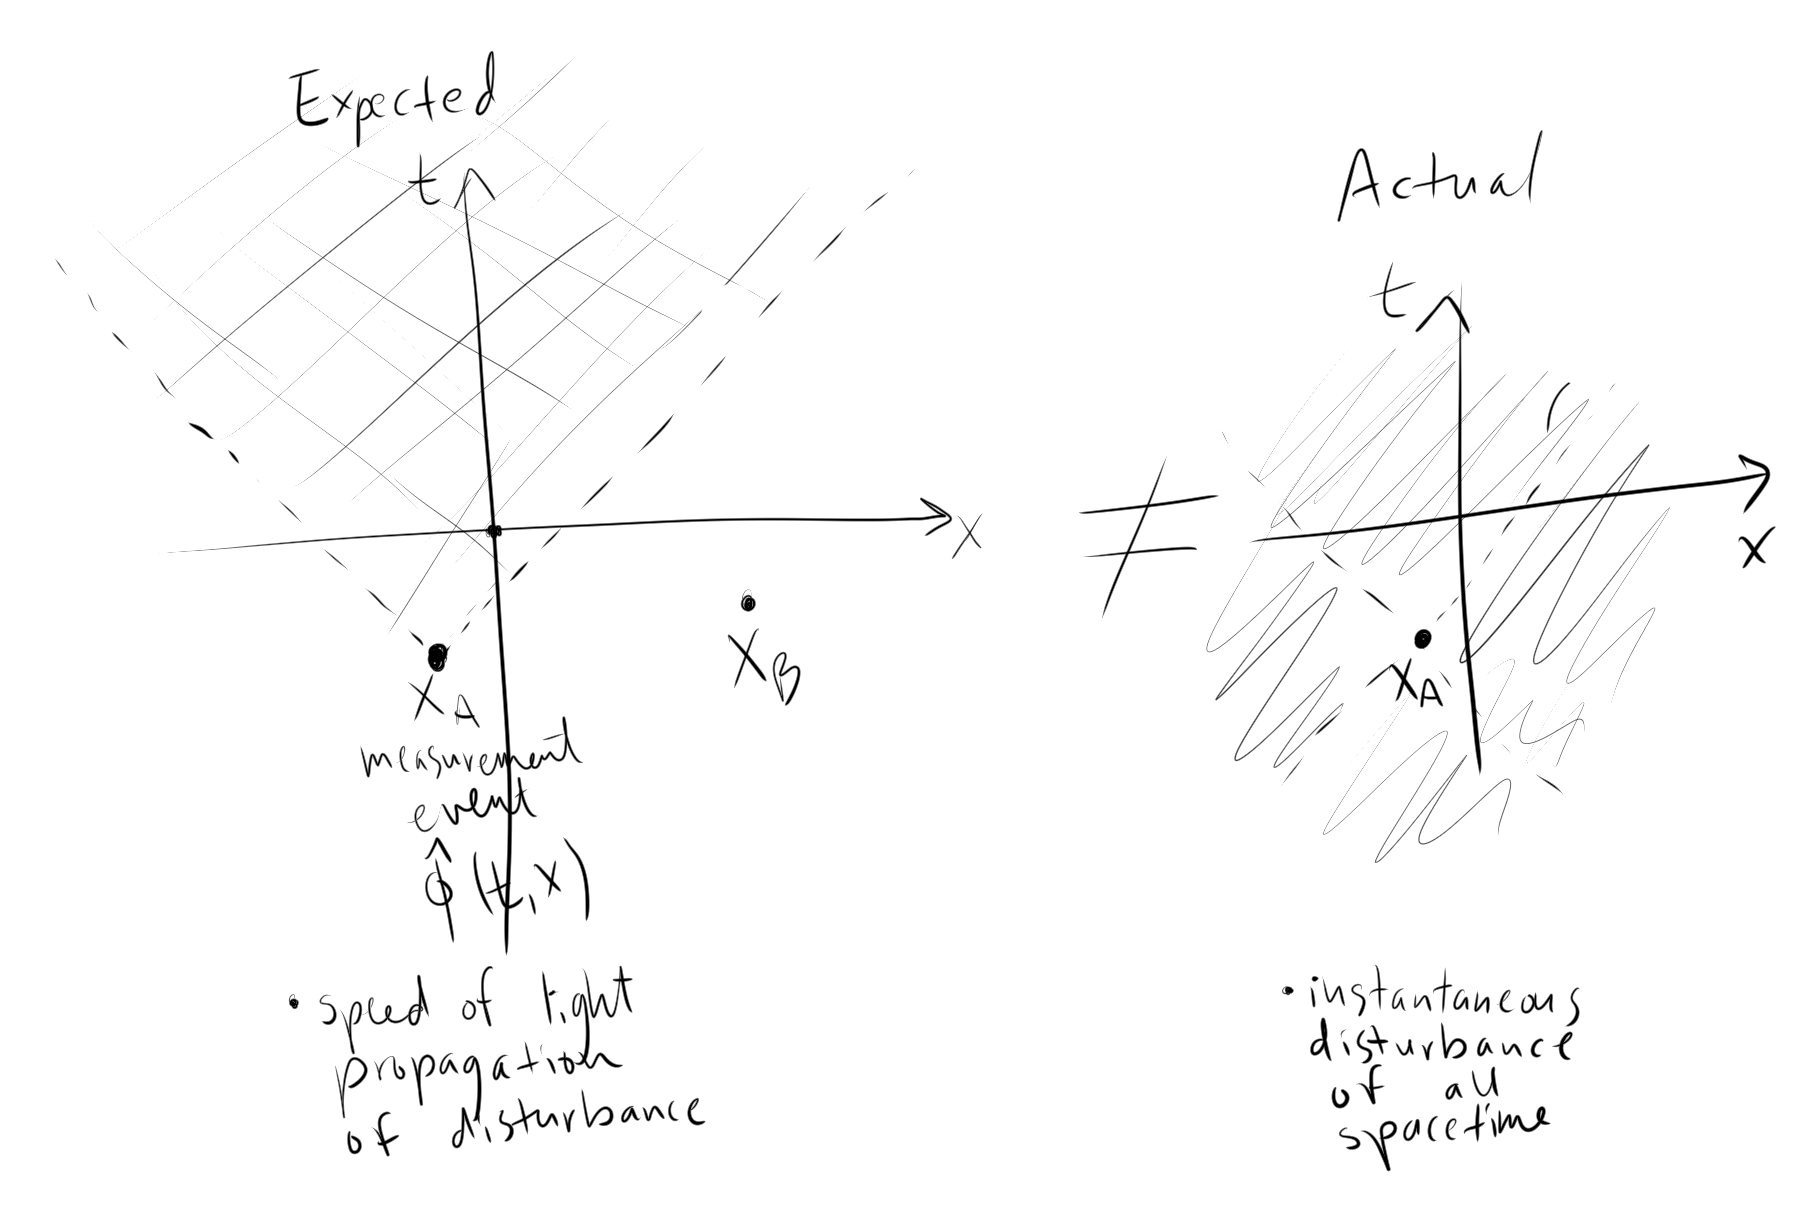
\includegraphics[scale=0.3]{images/lightcone.png}
	\caption{Sketch of expected propagation of information (at the speed of light) due to measurement event of the field $\hat{\phi}(t,x)$.}
\end{figure}

\noindent The result is that no information may be transmitted via the field across a space-like interval ($(x_A - x_B)^2 < 0$). \\

\noindent Now, we have to agree on which quantities are observable, and a natural guess is to study the correlation function
\begin{equation}
\bra{0} \hat{\phi}(x^0,x) \hat{\phi}(y^0,y) \ket{0}.
\end{equation}

\noindent This is unfortunately wrong, since the correlation function has no operational meaning, and can not be directly measured, since the field operators are not Hermitian, in general. \\

\noindent \textbf{Digression: Interference experiment} \\

\noindent To study correlation functions which can be measured in the lab via experiment, consider the following interference experiment set up with a Klein-Gordon field with auxiliary modes of light used to perform measurements and generate results. \\

\begin{figure}[H]
	\centering
	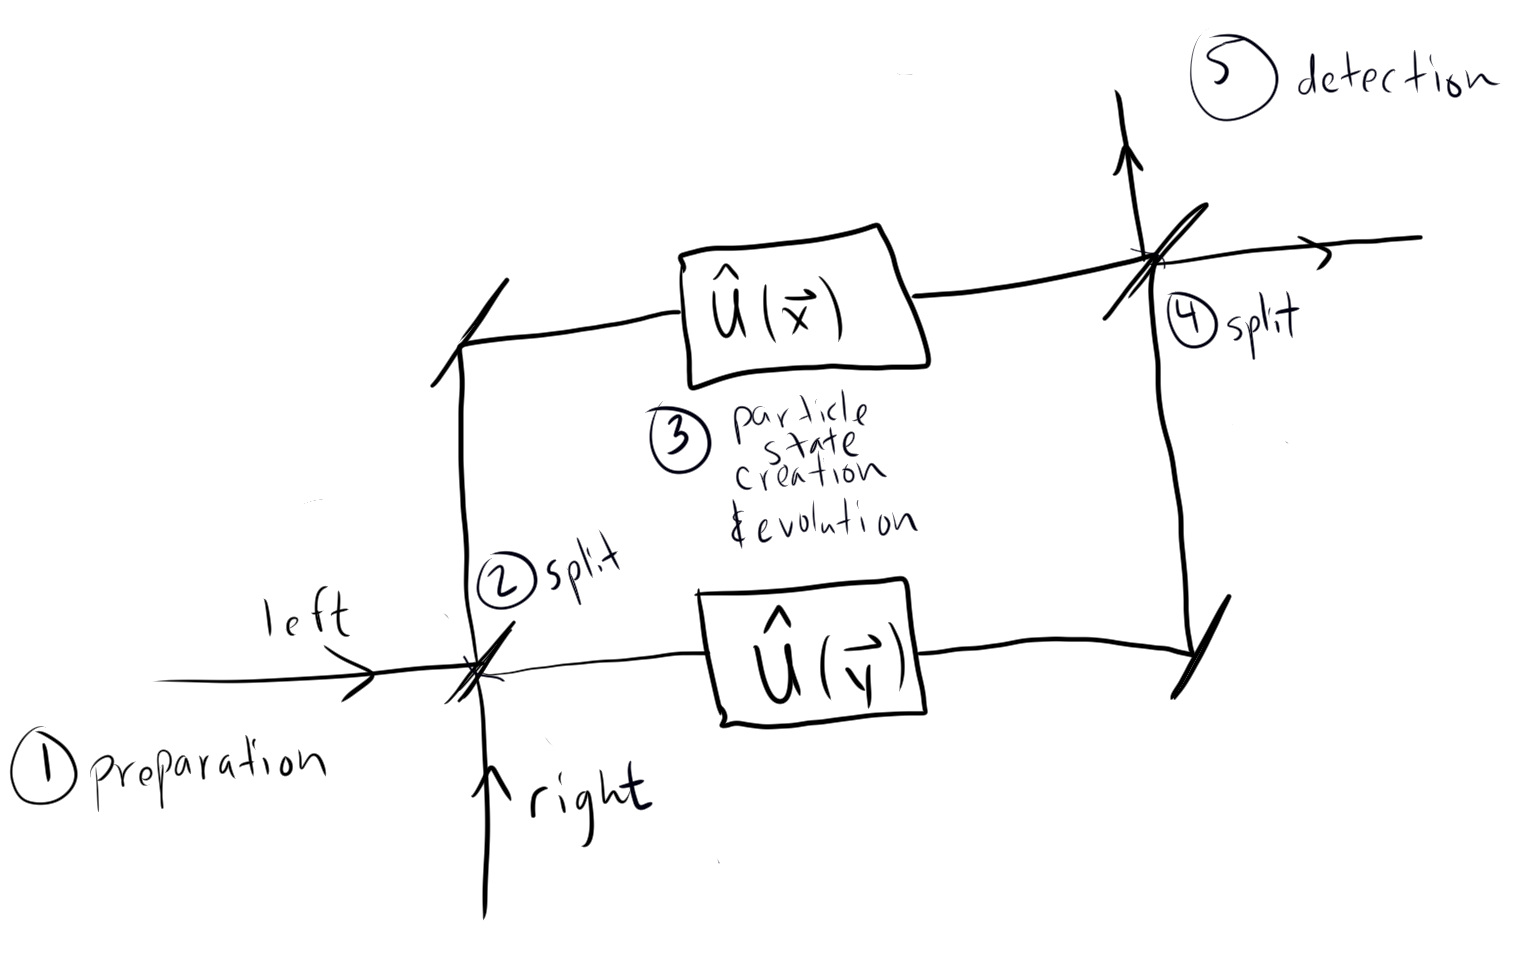
\includegraphics[scale=0.4]{images/interference.png}
	\caption{Schematic of experiment to measure the correlation of two spacetime locations and the Klein-Gordon field under measurement.}
\end{figure}

\begin{enumerate}
\item Prepare the field and auxiliary system (left and right) in the vacuum state
	\begin{equation}
	\ket{0}_{field} \ket{0}_{left} \ket{0}_{right}.
	\end{equation}
\item Apply the Hadamard gate (beam splitter) to the left and right auxiliary states
	\begin{equation}
	\ket{0}_{field} \left( \frac{1}{\sqrt{2}} \left( \ket{0}_{left} \ket{1}_{right} + \ket{1}_{left} \ket{0}_{right} \right) \right).
	\end{equation}
\item Create a particle at $\textbf{x}$ or $\textbf{y}$ via the unitary operator
	\begin{equation}
	\hat{U}(\textbf{x}) \otimes \ket{1}\bra{1}_{left} \otimes \mathbb{I}_{right} + \hat{U}(\textbf{y}) \otimes \mathbb{I}_{left} \ket{1}\bra{1}_{right}
	\end{equation}
	Applied to the state in \textbf{Step 2}, which evolves to the state (dropping "left" and "right" labels)
	\begin{equation}
	\frac{1}{\sqrt{2}} \left( \hat{U}(\textbf{y}) \ket{0}_{field} \ket{0 \, 1} + \hat{U}(\textbf{x}) \ket{0}_{field} \ket{1 \, 0} \right)
	\end{equation}
\item Apply a second beam splitter to the auxiliary states to check for interference in the final state
	\begin{equation}
	\frac{1}{2} \left( \hat{U}(\textbf{x}) + \hat{U}(\textbf{y}) \right) \ket{0}_{field} \ket{0 \, 1} + \frac{1}{2} \left( \hat{U}(\textbf{x}) - \hat{U}(\textbf{y}) \right) \ket{0}_{field} \ket{1 \, 0}
	\end{equation}
\item Detect auxiliary states $\ket{0 \, 1}$ and $\ket{1 \, 0}$.  
\end{enumerate}

\noindent The probability of measuring one of the states, $\ket{0 \, 1}$, for example, is 
\begin{align}
\mathcal{P}(\ket{0 \, 1}) &= \frac{1}{4} \bra{0}_{field} \left( \hat{U}^\dagger(\textbf{x}) + \hat{U}^\dagger(\textbf{y}) \right) \left( \hat{U}(\textbf{x}) + \hat{U}(\textbf{y}) \right)  \ket{0}_{field} \\
&= \frac{1}{2} + \frac{1}{2} Re \left[ \bra{0}_{field} \hat{U}^\dagger(\textbf{x}) \hat{U}(\textbf{y}) \ket{0}_{field} \right] \\
&= \frac{1}{2} + \frac{1}{2} Re \left[ \bra{0}_{field} e^{-i \epsilon \hat{\phi}(\textbf{x})} e^{i \epsilon \hat{\phi}(\textbf{y})} \ket{0}_{field} \right] \\
\mathcal{P}(\ket{0 \, 1}) &= \frac{1}{2} + \frac{1}{2} Re \left[ \bra{0}_{field} e^{-i \epsilon \hat{\phi}(\textbf{x})+ i \epsilon \hat{\phi}(\textbf{y}) +\frac{1}{2} \epsilon^2 [ \hat{\phi}(\textbf{x}), \hat{\phi}(\textbf{y}) ] } \ket{0}_{field} \right] \\
\end{align}

\noindent Where the last line is gotten via the Baker-Campbell-Hausdorff relation, since the two fields operators do not necessarily commute, and the interference between the two measurement events is determined by whether the commutator is zero or nonzero, which is calculated \\
\begin{align}
[ \hat{\phi}(\textbf{x}), \hat{\phi}(\textbf{y}) ] &= \int \frac{d^3 p}{(2\pi)^3} \int \frac{d^3 q}{(2\pi)^3} \frac{1}{\sqrt{4 \omega_p \omega_q}} \left( [\hat{a}_p, \hat{a}_q^\dagger ] e^{-i \textbf{p} \cdot \textbf{x} + i \textbf{q} \cdot \textbf{y}} + [\hat{a}_p^\dagger, \hat{a}_q ] e^{i \textbf{p} \cdot \textbf{x} - i \textbf{q} \cdot \textbf{y}} \right) \\
&= \int \frac{d^3 p}{(2\pi)^3} \frac{1}{\sqrt{2 \omega_p}} \left( e^{-i \textbf{p} \cdot (\textbf{x}-\textbf{y})} - e^{i \textbf{p} \cdot (\textbf{x}-\textbf{y})} \right) \cdot \mathbb{I} \\
[ \hat{\phi}(\textbf{x}), \hat{\phi}(\textbf{y}) ] &= \Delta (\textbf{x} - \textbf{y}) \cdot \mathbb{I}
\end{align}

\noindent Where the commutation relation $[\hat{a}_p, \hat{a}_q^\dagger] = (2\pi)^3 \delta^{(3)} (p-q) \cdot \mathbb{I}$ is used, and the quantity $\Delta (\textbf{x} - \textbf{y})$, the \textbf{correlation function}, which is Lorentz invariant, must be zero when $\textbf{x}$ and $\textbf{y}$ are space-like separated, such that $(\textbf{x} - \textbf{y})^2 < 0$. \\

\noindent Consider the space-like separation, $(\textbf{x} - \textbf{y})^2 < 0$, and enter a reference frame where $\textbf{x} - \textbf{y} = (0, x-y)$, and the correlation function $\Delta (\textbf{x} - \textbf{y})$ becomes zero!
\begin{align}
\Delta (\textbf{x} - \textbf{y}) &= \frac{1}{2} \int \frac{d^3 p}{(2\pi)^3} \frac{1}{\sqrt{|p|^2+m^2}} \left( e^{i p \cdot (x-y)} - e^{-ip \cdot (x-y)} \right) \\
&= \frac{1}{2} \int \frac{d^3 p}{(2\pi)^3} \frac{1}{\sqrt{|p|^2+m^2}} \left( e^{i p \cdot (x-y)} - e^{ip \cdot (x-y)} \right) \\
\Delta (\textbf{x} - \textbf{y}) &= 0
\end{align}

\noindent Where the second line is gotten by applying the Lorentz transformation $(x-y) \rightarrow -(x-y)$, which is allowed for in a space-like interval. \\

\begin{figure}[H]
	\centering
	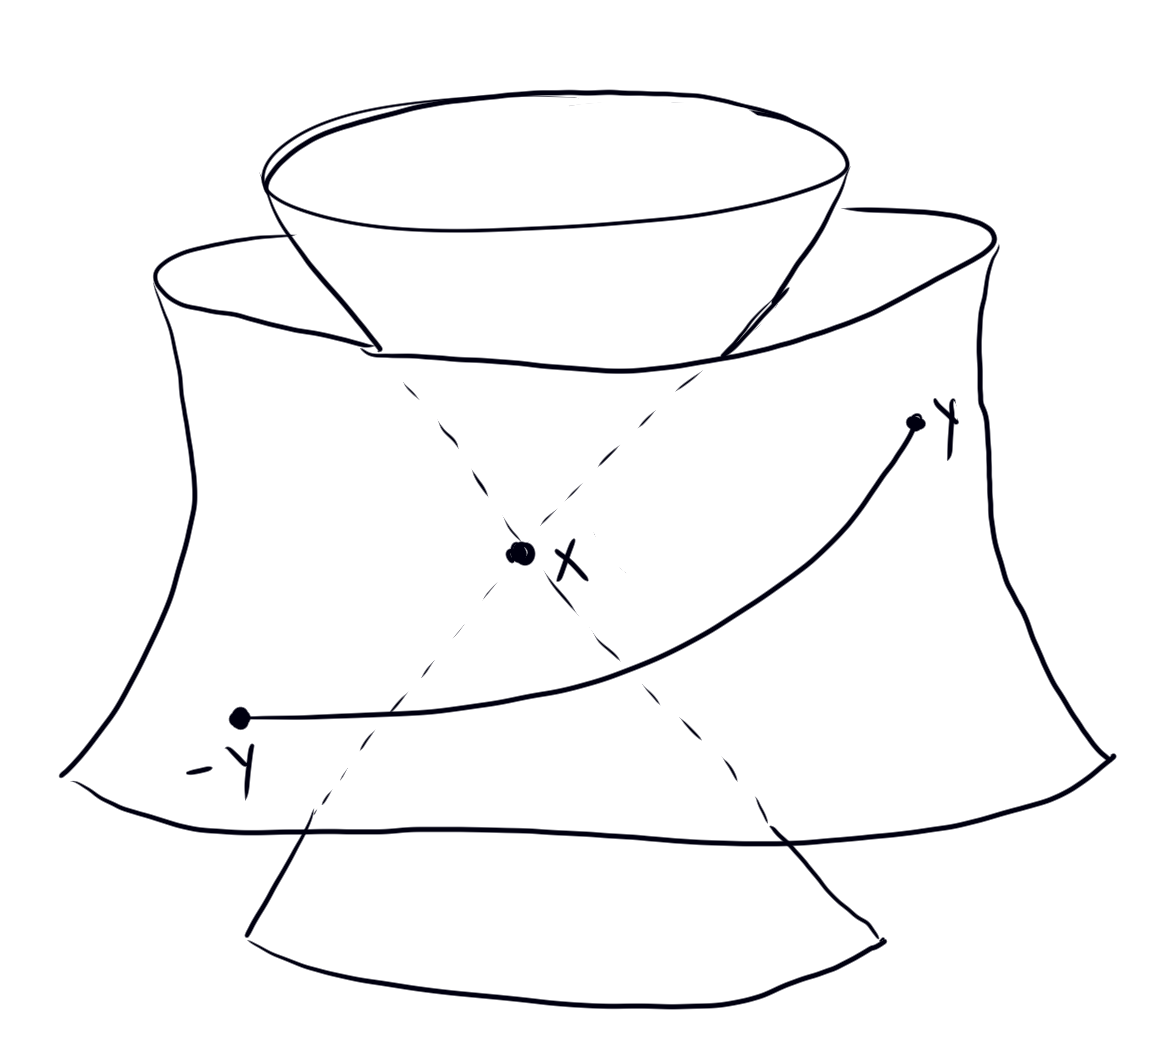
\includegraphics[scale=0.3]{images/inversion.png}
	\caption{Sketch of spatial inversion of spacetime location $\textbf{y}$.}
\end{figure}

\noindent Therefore, information does not travel faster than the speed of light, and the field operators respect causality when they are space-like separated! Note that this does not yet prove that the entire theory is causal. \\

\noindent As a side note, consider the case where the two field measurements are time-like separated, such that $(\textbf{x} - \textbf{y})^2 > 0$, and enter a reference frame where $\textbf{x} - \textbf{y} = (t, 0, 0, 0)$. In this reference frame of time-like separation, the correlation function can \textbf{not} be zero
\begin{align}
\Delta (\textbf{x} - \textbf{y}) &= \int \frac{d^3 p}{(2\pi)^3} \frac{1}{\sqrt{2 \omega_p}} \left( e^{-i\omega_p t} - e^{i\omega_p t} \right) \\
&= \frac{1}{4\pi^2} \int_m^{\infty} dE \, \sqrt{E^2 + m^2} e^{-iEt} \\
\Delta (\textbf{x} - \textbf{y}) &\sim e^{-imt} - e^{imt} \ne 0 .
\end{align}

\noindent Return to consider the (non-physical) two-point correlation function in a space-like interval
\begin{align}
D(\textbf{x}-\textbf{y}) &= \bra{0} \hat{\phi}(\textbf{x}) \hat{\phi}(\textbf{y}) \ket{0} \\
&= \int \frac{d^3 p}{(2\pi)^3} \frac{1}{2 \omega_p} e^{-i \textbf{p} \cdot (\textbf{x}-\textbf{y})} \\
&= \frac{1}{2} \int \frac{d^3 p}{(2\pi)^3} \frac{1}{\sqrt{|p|^2 + m^2}} e^{i p \cdot( x-y)} \\
&= \frac{m}{4\pi^2} \frac{1}{|x-y|} K_1(m|x-y|) \\
D(\textbf{x}-\textbf{y}) &\sim e^{-m|x-y|} \ne 0
\end{align}

\noindent Where $K_1(x)$ denotes the Hankel function. \\

\noindent So, when $\textbf{x}$ and $\textbf{y}$ are space-like separated, this correlation function can not be zero, and can therefore not carry any information, as it would have to travel faster than the speed of light. \\

\noindent An important application of the correlation function is the \textbf{Feynman propagator}, which is used later in perturbative expansions for describing interactions.
\begin{align}
    \Delta_F (\textbf{x} - \textbf{y}) &=
    \begin{cases}
      D(\textbf{x} - \textbf{y}), & x^0 > y^0 \\
      D(\textbf{y} - \textbf{x}), & x^0 < y^0
    \end{cases} \\
\Delta_F (\textbf{x} - \textbf{y}) &= \bra{0} \mathcal{T} [ \hat{\phi}(\textbf{x}) \hat{\phi}(\textbf{y}) ] \ket{0}
\end{align}

\noindent Where $\mathcal{T[\,]}$ is called the \textbf{time-ordering operator}
\begin{equation}
\mathcal{T} [ \hat{\phi}(\textbf{x}) \hat{\phi}(\textbf{y}) ] =
    \begin{cases}
      \hat{\phi}(\textbf{x}) \hat{\phi}(\textbf{y}), & x^0 > y^0 \\
      \hat{\phi}(\textbf{y}) \hat{\phi}(\textbf{x}), & x^0 < y^0
    \end{cases}
\end{equation}

\noindent Another important definition of the Feynman propagator is in terms of complex variables and contour integrals. \\

\noindent \textbf{Lemma:} 
\begin{align}
\Delta_F (\textbf{x} - \textbf{y}) &= \int \frac{d^4 p}{(2\pi)^4} \frac{i e^{-i \textbf{p} \cdot (\textbf{x}-\textbf{y})}}{|\textbf{p}|^2 - m^2 +i \epsilon} \\
&= \int \frac{d^3 p}{(2\pi)^3} \int_C \frac{d p^0}{2\pi} \frac{i e^{-i \textbf{p} \cdot (\textbf{x}-\textbf{y})}}{|\textbf{p}|^2 - m^2 +i \epsilon}
\end{align}

\noindent Where the integrand of the contour integral over the complex variable $p^0$ has two poles at $\pm i\epsilon$, and the contour is taken along the real $p^0$ axis, and closed in the upper or lower half-plane, depending on the value of $p^0$. \\

\begin{figure}[H]
	\centering
	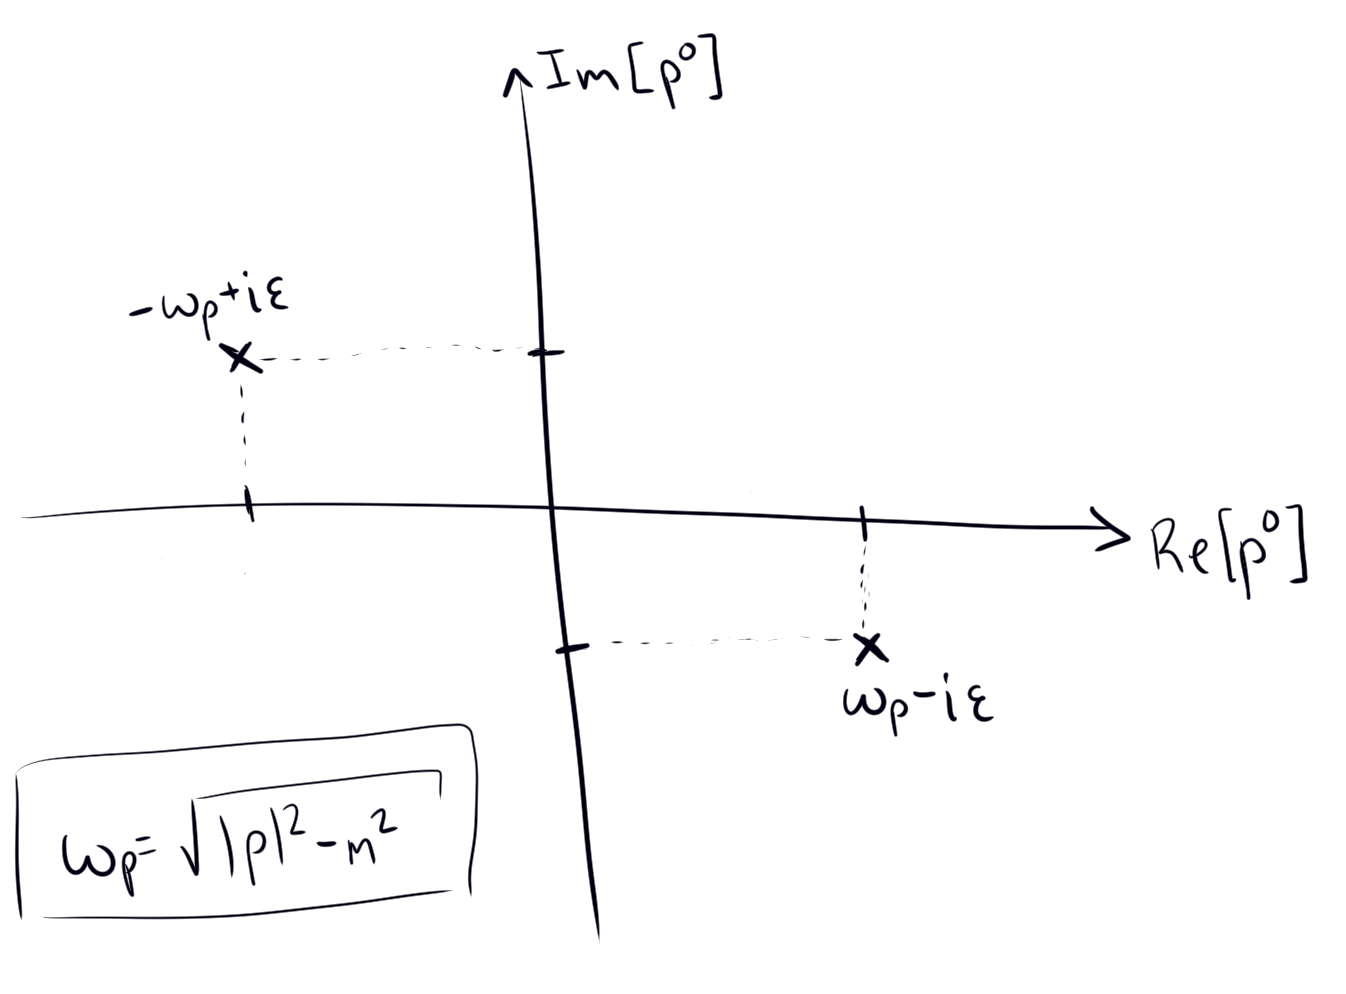
\includegraphics[scale=0.5]{images/poles.png}
	\caption{Poles of the Feynman propagator, where the contour may be taken in the upper half-plane for $t<0$, and in the lower half-plane for $t>0$, where $t=x^0-y_0$.}
\end{figure}

\noindent Lastly, an observation that the Feynman propagator, which is related thus far to the two-point correlation function, is also a Green's function (inverse of a differential operator) for the Klein-Gordon partial differential equation
\begin{align}
(\partial_0^2 - \nabla^2 + m^2) \Delta_F(\textbf{x} - \textbf{y}) &= -i \delta^{(4)} (\textbf{x} - \textbf{y}) \\
\sim \hat{\mathbb{L}} \cdot \hat{\mathbb{L}}^{-1} &= \mathbb{I}
\end{align}

\noindent Where the left-hand side is the product of a linear differential operator, the Klein-Gordon operator, and its inverse, the Feynman propagator, and the right-hand side of the equation is, in essence, the identity.